% ---
% title: Agent 的使用技巧
% date: 2026-10-22
% tag: Slides
% excerpt: 一场约 15 分钟的分享：把「用 coding agent」拆成三个环节——说清楚、放它做、盯结果。给上下文而不是让它猜，把大任务拆成可验证的小步，说清「完成」长什么样；让它读代码、独立的事并行、大改动先计划；最后读 diff、跑测试，错了改原因而不只是结果，并把反馈沉淀成规则。附四个反模式与开工前的检查清单。
% ---
% About 15 minutes: 开场 1 min，「说清楚」2.5 min，「放它做」2 min，
% 「盯结果」2.5 min，反模式与清单 2 min。三个环节各三条技巧，
% 每条一页；页面顶端的注释给出建议时长。图中文字只用 ASCII
% （TikZJax 用 Computer Modern 编译，没有中文字形）。
\documentclass[aspectratio=169]{beamer}
\usetikzlibrary{arrows.meta,positioning}
\definecolor{sig}{HTML}{1F5FAD}
\definecolor{hot}{HTML}{C0392B}
\definecolor{accent}{HTML}{C77C02}
\definecolor{soft}{HTML}{8C8C8C}
\definecolor{video}{HTML}{2E7D6B}

\title[Agent 使用技巧]{Agent 的使用技巧}
\subtitle{从一句话到一个可交付的结果}
\author{Xu Chen}
\date{October 2026}

\begin{document}

% 0:15
\begin{frame}
  \titlepage
\end{frame}

% 1:00
\begin{frame}{Agent 是你手的延伸，不是替你上班的员工}
  \begin{center}
  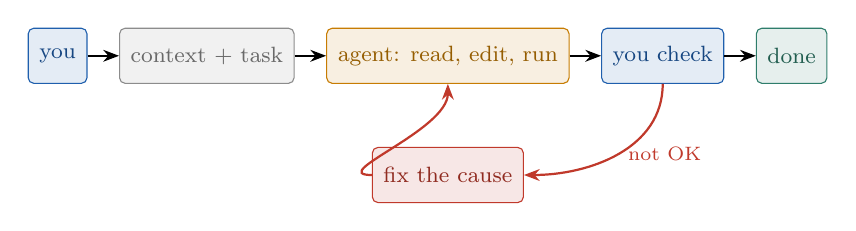
\begin{tikzpicture}[>={Stealth[length=2mm]}, font=\footnotesize, node distance=4mm,
      box/.style={draw=#1, fill=#1!12, text=#1!75!black, rounded corners=2pt, minimum height=7mm, inner sep=4pt}]
    \node[box=sig] (you) {you};
    \node[box=soft, right=of you] (ctx) {context + task};
    \node[box=accent, right=of ctx] (agent) {agent: read, edit, run};
    \node[box=sig, right=of agent] (check) {you check};
    \node[box=video, right=of check] (done) {done};
    \node[box=hot, below=8mm of agent] (fix) {fix the cause};
    \draw[thick, ->] (you) -- (ctx);
    \draw[thick, ->] (ctx) -- (agent);
    \draw[thick, ->] (agent) -- (check);
    \draw[thick, ->] (check) -- (done);
    \draw[thick, ->, hot] (check.south) to[out=270, in=0] node[right, font=\scriptsize] {not OK} (fix.east);
    \draw[thick, ->, hot] (fix.west) to[out=180, in=270] (agent.south);
  \end{tikzpicture}
  \end{center}
  \medskip
  一个 agent 只有三个旋钮：\textbf{上下文}（它知道什么）、\textbf{任务}（它要做什么）、
  \textbf{验收}（你怎么知道做对了）。它不会猜你的意图，只会做你说清楚、你能检查的事。
  所以用它的技巧，就是在这三个旋钮上各拧到位。
\end{frame}

% 0:30
\begin{frame}{三个环节，九条技巧}
  \begin{center}
  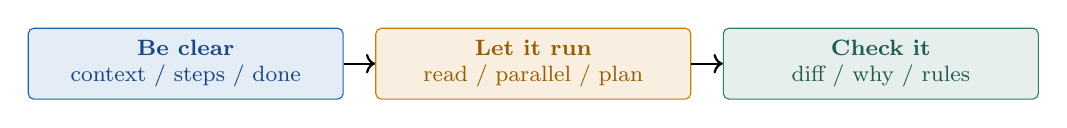
\begin{tikzpicture}[font=\footnotesize, node distance=4mm,
      box/.style={draw=#1, fill=#1!12, text=#1!75!black, rounded corners=2pt, minimum height=9mm, minimum width=40mm, inner sep=4pt, align=center}]
    \node[box=sig] (a) {\textbf{Be clear}\\context / steps / done};
    \node[box=accent, right=of a] (b) {\textbf{Let it run}\\read / parallel / plan};
    \node[box=video, right=of b] (c) {\textbf{Check it}\\diff / why / rules};
    \draw[thick, ->] (a) -- (b);
    \draw[thick, ->] (b) -- (c);
  \end{tikzpicture}
  \end{center}
  \medskip
  \begin{itemize}
    \item 大多数人只在「任务」上用力，却漏了上下文和验收——这正是 agent 出错的源头。
    \item 每个环节三条技巧，都是能立刻照做的动作，不是心态口号。
  \end{itemize}
\end{frame}

\section{说清楚}

% 0:50
\begin{frame}{技巧 1：给上下文，别让它猜}
  \begin{columns}[T]
    \begin{column}{0.48\textwidth}
      \textbf{\textcolor{hot}{它猜不着}}\\[2pt]
      「帮我改一下这个函数。」
      \begin{itemize}
        \item 哪个文件、哪个函数？
        \item 有哪些约束不能碰？
        \item 为什么要改？
      \end{itemize}
    \end{column}
    \begin{column}{0.52\textwidth}
      \textbf{\textcolor{video}{它照着做}}\\[2pt]
      「在 \texttt{src/foo.ts:120} 的 \texttt{Foo()} 里，
      同一个数组被循环读了两次；合并成一次。
      别改公共接口——有两处调用依赖它。
      原因：这一行在热路径上。」
    \end{column}
  \end{columns}
  \bigskip
  上下文 = \textbf{位置} + \textbf{约束（别动什么）} + \textbf{动机（为什么）}。
  三条里缺一条，它就用自己的默认值补上——而你多半不会喜欢那个默认值。
\end{frame}

% 0:50
\begin{frame}{技巧 2：大任务拆成可验证的小步}
  \begin{itemize}
    \item 一次只给一个想法；\textbf{每一步结束都有一个你能检查的产物}。
    \item 「重构认证系统」一步到位 → 几十个文件一起变，跑偏了都不知道从哪追。
    \item 拆成：先列改动点 → 你确认 → 逐文件改 → 每步跑一次测试。
  \end{itemize}
  \begin{center}
  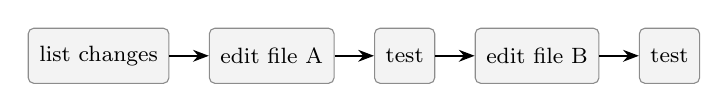
\begin{tikzpicture}[>={Stealth[length=2mm]}, font=\footnotesize, node distance=5mm,
      box/.style={draw=soft, fill=soft!10, rounded corners=2pt, minimum height=7mm, inner sep=4pt}]
    \node[box] (l) {list changes};
    \node[box, right=of l] (a) {edit file A};
    \node[box, right=of a] (t) {test};
    \node[box, right=of t] (b) {edit file B};
    \node[box, right=of b] (t2) {test};
    \draw[thick, ->] (l) -- (a);
    \draw[thick, ->] (a) -- (t);
    \draw[thick, ->] (t) -- (b);
    \draw[thick, ->] (b) -- (t2);
  \end{tikzpicture}
  \end{center}
  一大坨请求会漂移；小步让每一处偏离都被\alert{当场}抓住，而不是最后一起爆炸。
\end{frame}

% 0:40
\begin{frame}{技巧 3：说清「完成」长什么样}
  \begin{center}
  \alert{「改完跑 \texttt{npm test}，3 个新用例通过，不动 \texttt{public/} 下的任何文件。」}
  \end{center}
  \bigskip
  验收标准 = \textbf{跑哪个命令} + \textbf{预期输出} + \textbf{允许/禁止碰的东西}。
  \begin{itemize}
    \item 没有验收标准，「完成」就被 agent 自己定义——它往往定义成「看起来写完了」。
    \item 验收标准同时也是你的检查清单：做完照着验一遍就行。
  \end{itemize}
\end{frame}

\section{放它做}

% 0:40
\begin{frame}{技巧 4：让它读代码，别粘贴}
  \begin{itemize}
    \item Agent 搜索、读文件很快，还能顺着符号、引用一路跳转。\textbf{指向它，而不是喂给它}。
    \item 给 \texttt{文件:行号}、符号名、目录，它会自己去看；你粘贴反而又慢又容易截断关键上下文。
    \item 只粘贴它\alert{看不到}的东西：截图、运行日志、报错、外部网页。
  \end{itemize}
  \begin{center}
  \textcolor{soft}{\small 你只需留下结论，而不是把整个仓库塞进对话。}
  \end{center}
\end{frame}

% 0:40
\begin{frame}{技巧 5：独立的事并行}
  \begin{columns}[T]
    \begin{column}{0.55\textwidth}
      \begin{itemize}
        \item 互不依赖的活交给子 agent \textbf{并行}做：同时查三套候选方案、分头审不同文件。
        \item 你只收结论，不收「文件转储」。
        \item 判断标准：两件事之间有没有先后依赖？没有，就可以并行。
      \end{itemize}
    \end{column}
    \begin{column}{0.45\textwidth}
      \begin{center}
      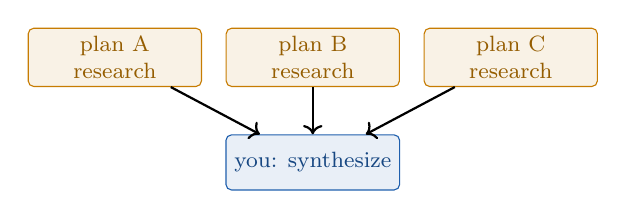
\begin{tikzpicture}[font=\footnotesize, node distance=3mm,
          box/.style={draw=accent, fill=accent!10, text=accent!75!black, rounded corners=2pt, minimum height=7mm, minimum width=22mm, align=center, inner sep=3pt}]
        \node[box] (q) {plan A\\research};
        \node[box, right=of q] (r) {plan B\\research};
        \node[box, right=of r] (s) {plan C\\research};
        \node[draw=sig, fill=sig!10, text=sig!75!black, rounded corners=2pt, minimum height=7mm, minimum width=22mm, align=center, inner sep=3pt, below=6mm of r] (y) {you: synthesize};
        \draw[thick, ->] (q) -- (y);
        \draw[thick, ->] (r) -- (y);
        \draw[thick, ->] (s) -- (y);
      \end{tikzpicture}
      \end{center}
    \end{column}
  \end{columns}
\end{frame}

% 0:40
\begin{frame}{技巧 6：大改动先计划}
  \begin{itemize}
    \item 多文件重构、新功能、改架构——先让它给\alert{方案}，你点头，再让它写代码。
    \item 对齐的是「\textbf{怎么做}」：动哪些文件、引入什么、迁移顺序是什么。
    \item 计划比代码便宜得多；先把路选对，省掉后面整段推倒重来。
  \end{itemize}
  \begin{center}
  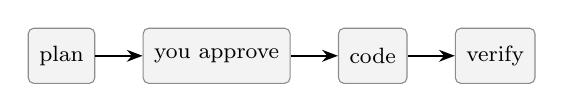
\begin{tikzpicture}[>={Stealth[length=2mm]}, font=\footnotesize, node distance=6mm,
      box/.style={draw=soft, fill=soft!10, rounded corners=2pt, minimum height=7mm, inner sep=4pt}]
    \node[box] (p) {plan};
    \node[box, right=of p] (y) {you approve};
    \node[box=accent, right=of y] (c) {code};
    \node[box=video, right=of c] (v) {verify};
    \draw[thick, ->] (p) -- (y);
    \draw[thick, ->] (y) -- (c);
    \draw[thick, ->] (c) -- (v);
  \end{tikzpicture}
  \end{center}
\end{frame}

\section{盯结果}

% 0:50
\begin{frame}{技巧 7：读 diff、跑测试，它报告你拍板}
  \begin{itemize}
    \item Agent 报告，\textbf{你}决定。它可能很自信地错，把错的也说得头头是道。
    \item 「能编译」$\neq$「对」；「测试通过」$\neq$「对」——测试本身可能没覆盖到。
    \item 读 \texttt{diff}、跑测试、盯关键路径；把它当一个熟练但会犯错的新人，不盲信。
  \end{itemize}
  \begin{center}
  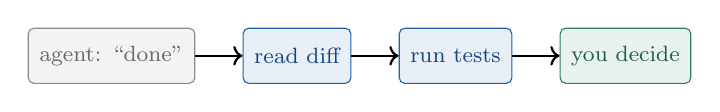
\begin{tikzpicture}[font=\footnotesize, node distance=6mm,
      box/.style={draw=#1, fill=#1!10, text=#1!75!black, rounded corners=2pt, minimum height=7mm, inner sep=4pt}]
    \node[box=soft] (c) {agent: ``done''};
    \node[box=sig, right=of c] (d) {read diff};
    \node[box=sig, right=of d] (t) {run tests};
    \node[box=video, right=of t] (y) {you decide};
    \draw[thick, ->] (c) -- (d);
    \draw[thick, ->] (d) -- (t);
    \draw[thick, ->] (t) -- (y);
  \end{tikzpicture}
  \end{center}
\end{frame}

% 0:40
\begin{frame}{技巧 8：改原因，不只是结果}
  \begin{columns}[T]
    \begin{column}{0.48\textwidth}
      \textbf{\textcolor{hot}{治标}}\\[2pt]
      「把第 5 行改对。」
      \begin{itemize}
        \item 它照最后一句重来，可能换个地方再犯同样的错。
      \end{itemize}
    \end{column}
    \begin{column}{0.52\textwidth}
      \textbf{\textcolor{video}{治本}}\\[2pt]
      「这里你用了同步 API，会阻塞事件循环；换成 \texttt{async}，
      并在调用处 \texttt{await} 它。」
      \begin{itemize}
        \item 给它\alert{原因}，它会顺着原因把整类问题一起修。
      \end{itemize}
    \end{column}
  \end{columns}
  \bigskip
  纠错时说清「\textbf{为什么错了}」，它就学到你的判断标准；只说「错了」，它只学会改这一处。
\end{frame}

% 0:40
\begin{frame}{技巧 9：把反馈沉淀成规则}
  \begin{itemize}
    \item 说过一遍的偏好，写进项目规则文件、记忆或偏好设置，\textbf{下次自动生效}，不用再讲第二遍。
    \item 例：「提交信息不要带 Co-Authored-By」「每次发版 bump \texttt{?v=}」「用 \texttt{x} 而不是 \texttt{y}」。
    \item 一遍遍口头纠正，是把自己变成 agent 的配置中心；沉淀下来，规则替你纠正。
  \end{itemize}
  \begin{center}
  \textcolor{soft}{\small 一次反馈 = 一次纠正；一条规则 = 从今往后每次都纠正。}
  \end{center}
\end{frame}

% 0:40
\begin{frame}{四个反模式}
  \begin{center}
  \footnotesize
  \begin{tabular}{lll}
    \toprule
    \textbf{反模式} & \textbf{结果} & \textbf{改法} \\
    \midrule
    任务模糊 & 它按默认值乱猜 & 补上位置、约束、动机（技巧 1） \\
    一大坨任务一次给 & 中途跑偏找不回 & 拆成可验证的小步（技巧 2） \\
    不检查就接受 & 自信地交付错的 & 读 diff、跑测试（技巧 7） \\
    原样重试 & 同样的错再来一遍 & 换思路、给原因（技巧 8） \\
    \bottomrule
  \end{tabular}
  \end{center}
  \medskip
  四个反模式，正好对应前面九条技巧里最常被跳过的那四条。
\end{frame}

% 0:40
\begin{frame}{开工前的检查清单}
  \begin{center}
  \footnotesize
  \begin{tabular}{ll}
    \toprule
    \textbf{开工前问自己} & \textbf{对应} \\
    \midrule
    它知道文件在哪、别动什么、为什么吗？ & 上下文（技巧 1） \\
    这一步结束时，我能验证吗？ & 拆小步（技巧 2） \\
    「完成」长什么样？ & 验收标准（技巧 3） \\
    哪些部分可以并行？ & 子 agent（技巧 5） \\
    要不要先看方案？ & 先计划（技巧 6） \\
    我准备读 diff、跑测试了吗？ & 盯结果（技巧 7） \\
    \bottomrule
  \end{tabular}
  \end{center}
  \bigskip
  \begin{center}
  \textbf{一句话：} Agent 的价值上限，由你给的\alert{上下文}和你做的\alert{检查}决定。
  \end{center}
\end{frame}

% 0:10
\begin{frame}[plain]
  \begin{center}
    {\Huge Thank you}

    \bigskip
    {\Large Questions?}
  \end{center}
\end{frame}

\end{document}
